\documentclass[11pt,aspectratio=169]{beamer}
\usetheme{Madrid}

% ======================= PACKAGES =======================
\usepackage{graphicx}
\usepackage{booktabs}
\usepackage{adjustbox}
\usepackage{multicol}
\usepackage{amsmath}
\usepackage{amssymb}
\usepackage{tikz}
\usetikzlibrary{arrows,shapes,positioning,shadows,trees}
\usepackage{listings}
\usepackage{xcolor}

% ======================= COLOR DEFINITIONS =======================
% Primary color scheme: Blue/Teal for Digital Finance
\definecolor{dfblue}{RGB}{0,102,204}
\definecolor{dfteal}{RGB}{0,153,153}
\definecolor{dfcyan}{RGB}{51,187,204}
\definecolor{dflightblue}{RGB}{153,204,255}
\definecolor{dflightblue2}{RGB}{173,214,255}
\definecolor{dflightblue3}{RGB}{193,224,255}
\definecolor{dflightblue4}{RGB}{213,234,255}

% Accent colors for finance applications
\definecolor{dfgreen}{RGB}{44, 160, 44}
\definecolor{dfred}{RGB}{214, 39, 40}
\definecolor{dforange}{RGB}{255, 127, 14}
\definecolor{dfgray}{RGB}{127, 127, 127}

% Utility colors
\definecolor{lightgray}{RGB}{240, 240, 240}
\definecolor{midgray}{RGB}{180, 180, 180}
\definecolor{codebg}{RGB}{245, 245, 245}

% ======================= THEME CUSTOMIZATION =======================
% Apply Digital Finance color scheme to Madrid theme
\setbeamercolor{palette primary}{bg=dflightblue3,fg=dfblue}
\setbeamercolor{palette secondary}{bg=dflightblue2,fg=dfblue}
\setbeamercolor{palette tertiary}{bg=dfteal,fg=white}
\setbeamercolor{palette quaternary}{bg=dfblue,fg=white}

\setbeamercolor{structure}{fg=dfblue}
\setbeamercolor{section in toc}{fg=dfblue}
\setbeamercolor{subsection in toc}{fg=dfteal}
\setbeamercolor{title}{fg=dfblue}
\setbeamercolor{frametitle}{fg=dfblue,bg=dflightblue3}
\setbeamercolor{block title}{bg=dflightblue2,fg=dfblue}
\setbeamercolor{block body}{bg=dflightblue4,fg=black}

% Remove navigation symbols for cleaner look
\setbeamertemplate{navigation symbols}{}

% Clean itemize/enumerate
\setbeamertemplate{itemize items}[circle]
\setbeamertemplate{enumerate items}[default]

% Margins for readability
\setbeamersize{text margin left=8mm,text margin right=8mm}

% ======================= LISTINGS CONFIGURATION =======================
% Python code style
\lstdefinestyle{pythonstyle}{
    language=Python,
    basicstyle=\ttfamily\footnotesize,
    keywordstyle=\color{dfblue}\bfseries,
    stringstyle=\color{dforange},
    commentstyle=\color{dfgray}\itshape,
    numberstyle=\tiny\color{dfgray},
    numbers=left,
    numbersep=5pt,
    backgroundcolor=\color{codebg},
    showspaces=false,
    showstringspaces=false,
    showtabs=false,
    frame=single,
    rulecolor=\color{midgray},
    tabsize=4,
    captionpos=b,
    breaklines=true,
    breakatwhitespace=false,
    escapeinside={(*@}{@*)},
    xleftmargin=10pt,
    xrightmargin=10pt
}

% Solidity code style
\lstdefinestyle{soliditystyle}{
    language=Java, % closest approximation
    basicstyle=\ttfamily\footnotesize,
    keywordstyle=\color{dfteal}\bfseries,
    stringstyle=\color{dforange},
    commentstyle=\color{dfgray}\itshape,
    numberstyle=\tiny\color{dfgray},
    numbers=left,
    numbersep=5pt,
    backgroundcolor=\color{codebg},
    showspaces=false,
    showstringspaces=false,
    showtabs=false,
    frame=single,
    rulecolor=\color{midgray},
    tabsize=2,
    captionpos=b,
    breaklines=true,
    breakatwhitespace=false,
    escapeinside={(*@}{@*)},
    xleftmargin=10pt,
    xrightmargin=10pt,
    morekeywords={pragma, contract, function, returns, public, private, view, pure, payable, address, uint256, mapping, event, modifier}
}

% Inline code command
\newcommand{\code}[1]{\texttt{\color{dfblue}#1}}

% ======================= CUSTOM COMMANDS =======================
% Bottom annotation (Madrid-style)
\newcommand{\bottomnote}[1]{%
\vfill
\vspace{-2mm}
\textcolor{dflightblue2}{\rule{\textwidth}{0.4pt}}
\vspace{1mm}
\footnotesize
\textbf{#1}
}

% Compact list spacing
\newcommand{\compactlist}{%
\setlength{\itemsep}{0pt}%
\setlength{\parskip}{0pt}%
\setlength{\parsep}{0pt}%
}

% Chart placeholder
\newcommand{\chartplaceholder}[2][5cm]{%
\begin{center}
\begin{adjustbox}{max width=0.95\textwidth, max height=#1}
\framebox[\textwidth][c]{%
\rule{0pt}{#1}%
\textcolor{midgray}{[#2]}%
}
\end{adjustbox}
\end{center}
}

% ======================= FINANCE NOTATION MACROS =======================
% Probability and statistics
\newcommand{\E}{\mathbb{E}} % Expected value
\newcommand{\Var}{\mathrm{Var}} % Variance
\newcommand{\Cov}{\mathrm{Cov}} % Covariance
\newcommand{\Prob}{\mathbb{P}} % Probability

% Distributions
\newcommand{\Normal}{\mathcal{N}} % Normal distribution
\newcommand{\Uniform}{\mathcal{U}} % Uniform distribution

% Returns and prices
\newcommand{\Ret}{R} % Return
\newcommand{\LogRet}{r} % Log return
\newcommand{\Price}{S} % Price/Stock price
\newcommand{\Strike}{K} % Strike price

% Options and derivatives
\newcommand{\CallPrice}{C} % Call option price
\newcommand{\PutPrice}{P} % Put option price
\newcommand{\Greeks}[1]{\mathit{#1}} % Greek letters

% Risk measures
\newcommand{\VaR}{\mathrm{VaR}} % Value at Risk
\newcommand{\CVaR}{\mathrm{CVaR}} % Conditional VaR
\newcommand{\Sharpe}{\mathrm{SR}} % Sharpe Ratio

% Time series
\newcommand{\AR}{\mathrm{AR}} % Autoregressive
\newcommand{\MA}{\mathrm{MA}} % Moving average
\newcommand{\GARCH}{\mathrm{GARCH}} % GARCH

% Blockchain/Crypto
\newcommand{\Hash}{\mathrm{Hash}} % Hash function
\newcommand{\Block}{\mathcal{B}} % Block
\newcommand{\Chain}{\mathcal{C}} % Chain

% Real numbers, integers
\newcommand{\R}{\mathbb{R}}
\newcommand{\Z}{\mathbb{Z}}
\newcommand{\N}{\mathbb{N}}

% ======================= TIKZ STYLES =======================
% Styles for finance-related diagrams
\tikzstyle{process} = [rectangle, minimum width=3cm, minimum height=1cm, text centered, draw=dfblue, fill=dflightblue4, thick]
\tikzstyle{decision} = [diamond, minimum width=3cm, minimum height=1cm, text centered, draw=dfteal, fill=dflightblue4, thick]
\tikzstyle{arrow} = [thick,->,>=stealth,color=dfblue]
\tikzstyle{blockchain} = [rectangle, rounded corners, minimum width=2.5cm, minimum height=1cm, text centered, draw=dfteal, fill=dflightblue3, thick]
\tikzstyle{transaction} = [circle, minimum size=0.8cm, text centered, draw=dforange, fill=dflightblue4, thick]

% ======================= FOOTER TEMPLATE =======================
\setbeamertemplate{footline}{
    \hbox{\begin{beamercolorbox}[wd=\paperwidth,ht=2.5ex,dp=1ex,leftskip=.5em,rightskip=.5em]{author in head/foot}
    \tiny
    \textbf{Digital Finance} \hfill
    Joerg Osterrieder \hfill
    \insertdate \hfill
    Page \insertframenumber{} / \inserttotalframenumber
    \end{beamercolorbox}}
}

% ======================= SECTION DIVIDER TEMPLATE =======================
\AtBeginSection[]{
\begin{frame}[plain]
\vfill
\centering
\begin{beamercolorbox}[sep=12pt,center]{title}
\usebeamerfont{title}\LARGE\insertsection\par
\end{beamercolorbox}
\vfill
\end{frame}
}


\title{Topic 2.4: Platform Economics}
\subtitle{Network Effects, Winner-Take-Most, and FinTech Business Models}
\author{Joerg Osterrieder}
\institute{Digital Finance}
\date{2025}

\begin{document}

% ==================== SLIDE 1: TITLE ====================
\begin{frame}
\titlepage
\end{frame}

% ==================== SLIDE 2: LEARNING OBJECTIVES ====================
\begin{frame}{Learning Objectives}
\begin{block}{By the end of this topic, you will be able to:}
\begin{enumerate}
\item \textbf{Define} what a platform is and distinguish it from traditional pipeline businesses
\item \textbf{Explain} direct and indirect network effects and Metcalfe's Law
\item \textbf{Analyze} winner-take-most dynamics and when markets ``tip''
\item \textbf{Evaluate} FinTech business models using revenue models and unit economics
\item \textbf{Assess} whether a FinTech's growth is sustainable or venture-subsidized
\item \textbf{Identify} regulatory moats and competitive barriers in financial services
\end{enumerate}
\end{block}

\vspace{3mm}
\begin{alertblock}{Key Competency}
Analyze a FinTech business model and assess its sustainability using platform economics concepts.
\end{alertblock}
\end{frame}

% ==================== SLIDE 3: PREREQUISITES/BACKGROUND ====================
\begin{frame}{Prerequisites: Economic Fundamentals}
\textbf{Before we begin, let's establish some foundational concepts:}

\vspace{3mm}
\begin{columns}[T]
\begin{column}{0.5\textwidth}
\textbf{Supply and Demand:}
\begin{itemize}
\item Markets match buyers (demand) with sellers (supply)
\item Prices adjust to balance the two
\item Traditional economics assumes linear relationships
\end{itemize}

\vspace{3mm}
\textbf{Business Models:}
\begin{itemize}
\item How a company creates value
\item How a company captures value (revenue)
\item Who pays and who benefits
\end{itemize}
\end{column}
\begin{column}{0.5\textwidth}
\textbf{Key Terms to Know:}
\begin{itemize}
\item \textbf{Value Chain}: Steps to create and deliver a product
\item \textbf{Marginal Cost}: Cost of producing one more unit
\item \textbf{Economies of Scale}: Lower costs at higher volumes
\item \textbf{Intermediary}: A middleman connecting parties
\end{itemize}

\vspace{3mm}
\textbf{Why This Matters:}\\
Platform economics \textit{changes} these traditional rules
\end{column}
\end{columns}
\end{frame}

% ==================== SLIDE 4: BACKGROUND - DIGITAL TRANSFORMATION ====================
\begin{frame}{Background: The Digital Transformation of Finance}
\begin{columns}[T]
\begin{column}{0.5\textwidth}
\textbf{Traditional Financial Services:}
\begin{itemize}
\item Banks manufacture and sell products
\item Physical branches, paper processes
\item Relationships built over time
\item High fixed costs, geographic limits
\end{itemize}

\vspace{3mm}
\textbf{Digital Disruption:}
\begin{itemize}
\item Software replaces physical infrastructure
\item APIs connect systems instantly
\item Data enables personalization
\item Global reach at near-zero marginal cost
\end{itemize}
\end{column}
\begin{column}{0.5\textwidth}
\begin{center}
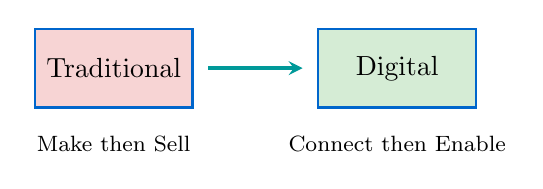
\begin{tikzpicture}[scale=0.8]
% Traditional
\node[process, fill=dfred!20, minimum width=2cm] (trad) at (0,2) {Traditional};
\node[font=\footnotesize] at (0,0.8) {Make then Sell};

% Arrow
\draw[arrow, very thick, dfteal] (1.5,2) -- (3,2);

% Digital
\node[process, fill=dfgreen!20, minimum width=2cm] (dig) at (4.5,2) {Digital};
\node[font=\footnotesize] at (4.5,0.8) {Connect then Enable};
\end{tikzpicture}
\end{center}

\vspace{2mm}
\textbf{Key Shifts:} Products to Platforms, Ownership to Access, Linear to Network

\begin{block}{The Platform Economy}
The most valuable companies today don't make things---they connect people and facilitate transactions.
\end{block}
\end{column}
\end{columns}
\end{frame}

% ==================== SLIDE 5: WHAT IS A PLATFORM? ====================
\begin{frame}{What is a Platform?}
\begin{columns}[T]
\begin{column}{0.5\textwidth}
\textbf{Definition:}\\
A business that creates value by facilitating exchanges between two or more interdependent groups

\vspace{3mm}
\textbf{Platform vs. Pipeline:}
\begin{itemize}
\item \textbf{Pipeline}: Linear value chain (make $\rightarrow$ sell)
\item \textbf{Platform}: Network orchestration (connect $\rightarrow$ facilitate)
\end{itemize}

\vspace{3mm}
\textbf{FinTech Examples:}
\begin{itemize}
\item Visa (merchants $\leftrightarrow$ cardholders)
\item Robinhood (traders $\leftrightarrow$ market makers)
\item LendingClub (borrowers $\leftrightarrow$ investors)
\end{itemize}
\end{column}
\begin{column}{0.5\textwidth}
\begin{center}
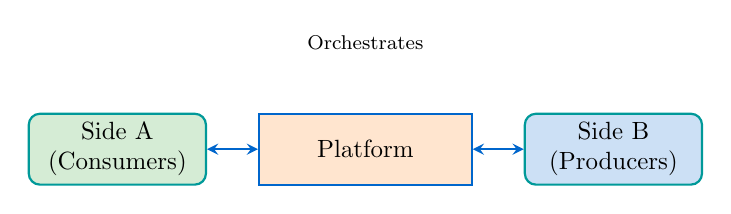
\begin{tikzpicture}[node distance=2cm, scale=0.9, transform shape]
% Platform model
\node (side1) [blockchain, fill=dfgreen!20, align=center] {Side A\\(Consumers)};
\node (platform) [process, right of=side1, xshift=1.5cm, fill=dforange!20] {Platform};
\node (side2) [blockchain, right of=platform, xshift=1.5cm, fill=dfblue!20, align=center] {Side B\\(Producers)};

% Arrows - bidirectional
\draw[thick, dfblue, stealth-stealth] (side1) -- (platform);
\draw[thick, dfblue, stealth-stealth] (platform) -- (side2);

% Value labels
\node[above of=platform, yshift=-0.5cm, font=\footnotesize] {Orchestrates};
\end{tikzpicture}
\end{center}

\vspace{5mm}
\begin{block}{Key Insight}
Platforms don't own the means of production---they own the means of \textbf{connection}.
\end{block}
\end{column}
\end{columns}
\end{frame}

% ==================== SLIDE 6: PIPELINE VS PLATFORM COMPARISON ====================
\begin{frame}{Pipeline vs. Platform: A Detailed Comparison}
\begin{center}
\begin{tabular}{p{3cm}p{5cm}p{5cm}}
\toprule
\textbf{Dimension} & \textbf{Pipeline (Traditional)} & \textbf{Platform (Digital)} \\
\midrule
\textbf{Value Creation} & Firm creates and sells products & Users create value for each other \\
\textbf{Assets} & Physical (branches, inventory) & Digital (software, data, networks) \\
\textbf{Growth} & Linear (more output = more cost) & Non-linear (network effects) \\
\textbf{Scalability} & Limited by physical capacity & Near-unlimited \\
\textbf{Competition} & Product features and price & Ecosystem size and quality \\
\textbf{Moat} & Proprietary technology, brand & Network effects, data, switching costs \\
\bottomrule
\end{tabular}
\end{center}

\vspace{5mm}
\textbf{Examples:}
\begin{itemize}
\item \textbf{Pipeline}: Traditional bank manufactures loans, sells to customers
\item \textbf{Platform}: LendingClub connects borrowers with investors who fund loans
\end{itemize}
\end{frame}

% ==================== SLIDE 7: NETWORK EFFECTS INTRODUCTION ====================
\begin{frame}{Network Effects: The Core Mechanism}
\begin{columns}[T]
\begin{column}{0.5\textwidth}
\textbf{What Are Network Effects?}\\
When the value of a product or service \textit{increases} as more people use it

\vspace{3mm}
\textbf{Direct Network Effects:}\\
More users $\rightarrow$ more value for each user

\vspace{2mm}
\textit{Example}: Venmo---more friends on the platform = more utility for you

\vspace{5mm}
\textbf{Indirect (Cross-Side) Network Effects:}\\
More users on Side A $\rightarrow$ more value for Side B

\vspace{2mm}
\textit{Example}: More Visa cardholders $\rightarrow$ merchants want to accept Visa
\end{column}
\begin{column}{0.5\textwidth}
\begin{block}{Metcalfe's Law}
Network value $\propto$ n$^2$\\
(where n = number of users)

\vspace{2mm}
\textbf{Implication}:\\
Doubling users quadruples value
\end{block}

\begin{alertblock}{Critical Mass}
Networks often have a ``tipping point''---below it, collapse; above it, dominance
\end{alertblock}

\textit{This is why platforms grow aggressively early on}
\end{column}
\end{columns}
\end{frame}

% ==================== SLIDE 8: METCALFE'S LAW VISUALIZED ====================
\begin{frame}{Metcalfe's Law: Why Networks Are Powerful}
\begin{columns}[T]
\begin{column}{0.5\textwidth}
\textbf{The Mathematics:}
\begin{itemize}
\item With \textbf{n} users, potential connections = $\frac{n(n-1)}{2}$
\item Approximately n$^2$/2 connections
\item Value grows \textbf{exponentially}, not linearly
\end{itemize}

\vspace{3mm}
\textbf{Practical Example:}
\begin{center}
\begin{tabular}{ccc}
\toprule
\textbf{Users} & \textbf{Connections} & \textbf{Relative Value} \\
\midrule
10 & 45 & 1x \\
20 & 190 & 4.2x \\
50 & 1,225 & 27x \\
100 & 4,950 & 110x \\
\bottomrule
\end{tabular}
\end{center}
\end{column}
\begin{column}{0.5\textwidth}
\begin{center}
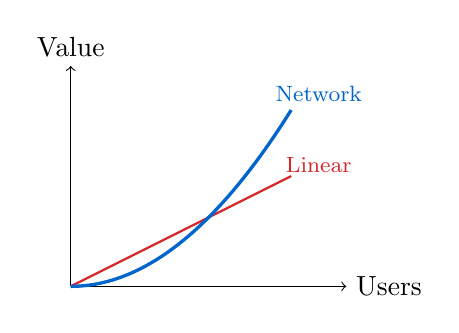
\begin{tikzpicture}[scale=0.7]
% Axes
\draw[->] (0,0) -- (5,0) node[right] {Users};
\draw[->] (0,0) -- (0,4) node[above] {Value};

% Linear growth
\draw[dfred, thick] (0,0) -- (4,2);
\node[dfred, font=\footnotesize] at (4.5,2.2) {Linear};

% Network growth (quadratic)
\draw[dfblue, very thick, domain=0:4, samples=50] plot (\x, {0.2*\x*\x});
\node[dfblue, font=\footnotesize] at (4.5,3.5) {Network};
\end{tikzpicture}
\end{center}

\begin{block}{Key Insight}
This is why the largest platforms (Visa, Uber, Airbnb) are worth so much---each new user adds value for \textit{all} existing users.
\end{block}
\end{column}
\end{columns}
\end{frame}

% ==================== SLIDE 9: TYPES OF NETWORK EFFECTS ====================
\begin{frame}{Types of Network Effects in FinTech}
\begin{center}
\begin{tabular}{p{3cm}p{4.5cm}p{4.5cm}}
\toprule
\textbf{Type} & \textbf{Description} & \textbf{FinTech Example} \\
\midrule
\textbf{Direct} & Same-side: users attract users & Venmo (peer payments), Zelle \\
\textbf{Indirect (Cross-side)} & One side attracts the other & Visa (cardholders $\leftrightarrow$ merchants) \\
\textbf{Data Network Effects} & More users = better algorithms & Credit Karma (better recommendations) \\
\textbf{Ecosystem Effects} & Third parties build on platform & Stripe (developer tools ecosystem) \\
\bottomrule
\end{tabular}
\end{center}

\vspace{5mm}
\begin{alertblock}{Critical Question for Any FinTech}
Does this company have \textbf{real} network effects, or just \textbf{growth}?\\
\vspace{2mm}
\textit{Growth without network effects is just expensive customer acquisition.}
\end{alertblock}
\end{frame}

% ==================== SLIDE 10: CHICKEN AND EGG PROBLEM ====================
\begin{frame}{The Chicken-and-Egg Problem}
\begin{center}
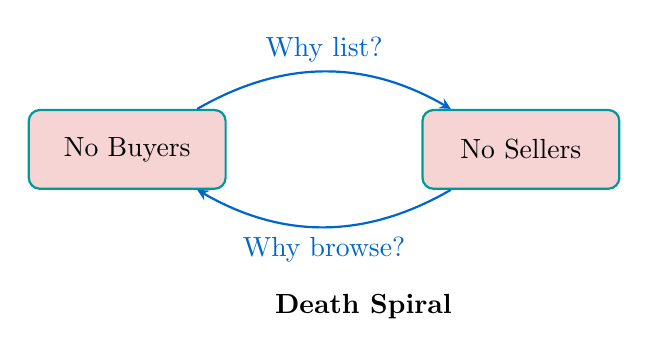
\begin{tikzpicture}[node distance=3cm]
% Chicken-egg cycle
\node (no_buyers) [blockchain, fill=dfred!20] {No Buyers};
\node (no_sellers) [blockchain, right of=no_buyers, xshift=2cm, fill=dfred!20] {No Sellers};

\draw[arrow, bend left=30] (no_buyers) to node[above] {Why list?} (no_sellers);
\draw[arrow, bend left=30] (no_sellers) to node[below] {Why browse?} (no_buyers);

\node[below of=no_buyers, xshift=3cm, yshift=1cm] {\textbf{Death Spiral}};
\end{tikzpicture}
\end{center}

\vspace{5mm}
\textbf{Platform Launch Strategies:}
\begin{columns}[T]
\begin{column}{0.33\textwidth}
\textbf{Subsidize one side}\\
PayPal paid users \$10 to sign up
\end{column}
\begin{column}{0.33\textwidth}
\textbf{Single-player mode}\\
Venmo: useful even alone (payment tracking)
\end{column}
\begin{column}{0.33\textwidth}
\textbf{Seed supply}\\
Some apps create initial content/profiles
\end{column}
\end{columns}
\end{frame}

% ==================== SLIDE 11: CRITICAL MASS ====================
\begin{frame}{Critical Mass: The Tipping Point}
\begin{columns}[T]
\begin{column}{0.5\textwidth}
\textbf{Definition:}\\
The minimum number of users needed for a network to become self-sustaining

\vspace{3mm}
\textbf{Below Critical Mass:}
\begin{itemize}
\item Users leave faster than they join
\item Value proposition is weak
\item Requires constant subsidies
\end{itemize}

\vspace{3mm}
\textbf{Above Critical Mass:}
\begin{itemize}
\item Organic growth accelerates
\item Network effects compound
\item Winner-take-most dynamics begin
\end{itemize}
\end{column}
\begin{column}{0.5\textwidth}
\begin{center}
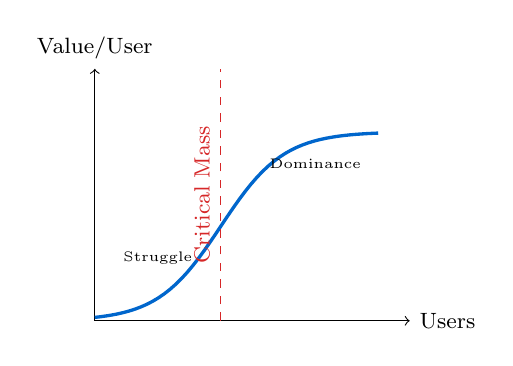
\begin{tikzpicture}[scale=0.8]
% Axes
\draw[->] (0,0) -- (5,0) node[right, font=\footnotesize] {Users};
\draw[->] (0,0) -- (0,4) node[above, font=\footnotesize] {Value/User};

% S-curve
\draw[dfblue, very thick, domain=0:4.5, samples=50] plot (\x, {3/(1+exp(-2*(\x-2)))});

% Critical mass line
\draw[dfred, dashed] (2,0) -- (2,4);
\node[dfred, font=\footnotesize, rotate=90] at (1.7,2) {Critical Mass};

% Labels
\node[font=\tiny] at (1,1) {Struggle};
\node[font=\tiny] at (3.5,2.5) {Dominance};
\end{tikzpicture}
\end{center}

\begin{block}{FinTech Implication}
This is why FinTechs raise large amounts of venture capital---to reach critical mass before running out of money.
\end{block}
\end{column}
\end{columns}
\end{frame}

% ==================== SLIDE 12: WINNER TAKE MOST ====================
\begin{frame}{Winner-Take-Most Dynamics}
\begin{columns}[T]
\begin{column}{0.5\textwidth}
\textbf{When Markets Tip:}
\begin{itemize}
\item Strong network effects
\item High multi-homing costs
\item Standardization benefits
\item Data advantages compound
\end{itemize}

\vspace{3mm}
\textbf{FinTech Examples:}
\begin{itemize}
\item Payments: Visa/Mastercard duopoly
\item Stock trading: NYSE dominance
\item Crypto smart contracts: Ethereum
\end{itemize}
\end{column}
\begin{column}{0.5\textwidth}
\begin{block}{Multi-Homing Prevents Tipping}
When users easily use multiple platforms:
\begin{itemize}
\item Less lock-in
\item Competition persists
\item Margins compress
\end{itemize}

\vspace{2mm}
\textbf{Example}: Drivers on Uber AND Lyft
\end{block}
\end{column}
\end{columns}

\vspace{3mm}
\begin{alertblock}{Key Question}
Does this FinTech's market tip, or does competition persist?
\end{alertblock}
\end{frame}

% ==================== SLIDE 13: MULTI-HOMING EXPLAINED ====================
\begin{frame}{Multi-Homing: The Competition Preserver}
\textbf{Definition:} When users can easily use multiple competing platforms simultaneously

\begin{columns}[T]
\begin{column}{0.5\textwidth}
\textbf{Low Multi-Homing Costs:}
\begin{itemize}
\item Easy to switch or use both
\item Competition remains intense
\item No clear winner emerges
\item Prices stay low
\end{itemize}

\vspace{2mm}
\textbf{Examples:}
\begin{itemize}
\item Ride-sharing: Uber vs. Lyft
\item Food delivery: DoorDash vs. Uber Eats
\item BNPL: Klarna vs. Afterpay
\end{itemize}
\end{column}
\begin{column}{0.5\textwidth}
\textbf{High Multi-Homing Costs:}
\begin{itemize}
\item Expensive to switch
\item Users commit to one platform
\item Market tips to winner
\item Pricing power follows
\end{itemize}

\vspace{2mm}
\textbf{Examples:}
\begin{itemize}
\item Payment networks: Visa/MC
\item Enterprise software: Stripe integration
\item Operating systems: iOS vs. Android
\end{itemize}
\end{column}
\end{columns}

\vspace{3mm}
\textbf{Strategic Implication:} Successful platforms try to \textit{increase} switching costs
\end{frame}

% ==================== SLIDE 14: FINTECH BUSINESS MODEL CANVAS ====================
\begin{frame}{FinTech Business Model Canvas}
\begin{center}
\begin{tabular}{|p{3cm}|p{4cm}|p{4cm}|}
\hline
\textbf{Element} & \textbf{Questions} & \textbf{Examples} \\
\hline
\textbf{Value Proposition} & What pain point? Better than alternatives how? & Speed, cost, access, UX \\
\hline
\textbf{Revenue Model} & Transaction fees? Subscription? Spread? Data? & 2.9\% + \$0.30, \$10/mo \\
\hline
\textbf{Cost Structure} & CAC? Infrastructure? Regulatory? & Marketing, cloud, compliance \\
\hline
\textbf{Network Effects} & Direct? Indirect? Data flywheel? & User-to-user, merchant-consumer \\
\hline
\textbf{Moat} & What prevents competition? & Switching costs, data, regulatory \\
\hline
\textbf{Scalability} & Marginal cost of growth? & Near-zero (software) vs. human-dependent \\
\hline
\end{tabular}
\end{center}

\vspace{3mm}
\textbf{Use this framework to analyze any FinTech company systematically.}
\end{frame}

% ==================== SLIDE 15: REVENUE MODELS OVERVIEW ====================
\begin{frame}{Revenue Models in FinTech}
\begin{columns}[T]
\begin{column}{0.5\textwidth}
\textbf{Transaction-Based:}
\begin{itemize}
\item \textbf{Interchange}: Card-based revenue
\item \textbf{Spread}: Bid-ask, FX markup
\item \textbf{Percentage fees}: 2.9\% of payment
\item \textbf{Flat fees}: \$0.30 per transaction
\end{itemize}

\vspace{2mm}
\textbf{Subscription:}
\begin{itemize}
\item \textbf{Premium features}: Robinhood Gold
\item \textbf{B2B SaaS}: Stripe Atlas
\item \textbf{Membership}: Amazon Prime
\end{itemize}
\end{column}
\begin{column}{0.5\textwidth}
\textbf{Interest/Float:}
\begin{itemize}
\item \textbf{Deposit spread}: Earn 5\%, pay 1\%
\item \textbf{Lending margin}: Borrow low, lend high
\item \textbf{Float}: Hold funds, earn interest
\end{itemize}

\vspace{2mm}
\textbf{Data/Ecosystem:}
\begin{itemize}
\item \textbf{PFOF}: Payment for order flow
\item \textbf{Cross-sell}: Land and expand
\item \textbf{Data licensing}: Aggregate insights
\end{itemize}
\end{column}
\end{columns}

\vspace{3mm}
\begin{block}{Key Insight}
Most successful FinTechs combine \textbf{multiple} revenue streams for resilience.
\end{block}
\end{frame}

% ==================== SLIDE 16: UNIT ECONOMICS ====================
\begin{frame}{Unit Economics: CAC, LTV, and Payback}
\begin{columns}[T]
\begin{column}{0.5\textwidth}
\textbf{Key Metrics Defined:}
\begin{itemize}
\item \textbf{CAC}: Customer Acquisition Cost\\
\textit{Total marketing spend / new customers}
\item \textbf{LTV}: Lifetime Value\\
\textit{Total revenue from a customer over time}
\item \textbf{Payback}: Months to recover CAC\\
\textit{CAC / monthly revenue per customer}
\item \textbf{Churn}: \% customers leaving per period
\end{itemize}

\vspace{2mm}
\textbf{Healthy Benchmarks:}
\begin{itemize}
\item LTV/CAC $>$ 3x
\item Payback $<$ 18 months
\item Churn $<$ 5\% annual (B2B)
\end{itemize}
\end{column}
\begin{column}{0.5\textwidth}
\begin{block}{FinTech CAC Challenges}
\begin{itemize}
\item Trust required for financial products
\item Regulatory constraints on marketing
\item High-intent keywords expensive
\item Referral programs costly
\end{itemize}
\end{block}

\vspace{2mm}
\textbf{Typical FinTech CACs:}\\
Neobank: \$100-300\\
Trading app: \$50-150\\
B2B SaaS: \$500-2,000
\end{column}
\end{columns}
\end{frame}

% ==================== SLIDE 17: UNIT ECONOMICS EXAMPLE ====================
\begin{frame}{Unit Economics: A Worked Example}
\textbf{Scenario:} A neobank acquiring customers

\begin{columns}[T]
\begin{column}{0.5\textwidth}
\textbf{Given:}
\begin{itemize}
\item CAC = \$200 (marketing cost per customer)
\item Monthly revenue = \$15 per customer
\item Average customer lifespan = 3 years
\item Monthly churn = 2.8\%
\end{itemize}

\vspace{3mm}
\textbf{Calculations:}
\begin{itemize}
\item LTV = \$15 $\times$ 36 months = \$540
\item LTV/CAC = \$540 / \$200 = \textbf{2.7x}
\item Payback = \$200 / \$15 = \textbf{13.3 months}
\end{itemize}
\end{column}
\begin{column}{0.5\textwidth}
\begin{alertblock}{Assessment}
\begin{itemize}
\item LTV/CAC 2.7x: \textcolor{dforange}{Below 3x threshold}
\item Payback 13.3 mo: \textcolor{dfgreen}{Within 18 months}
\end{itemize}

\vspace{2mm}
\textbf{Verdict}: Borderline healthy---needs to either:
\begin{itemize}
\item Reduce CAC (improve marketing efficiency)
\item Increase LTV (add products, reduce churn)
\end{itemize}
\end{alertblock}
\end{column}
\end{columns}

\vspace{3mm}
\textbf{Key Insight:} Unit economics determine long-term viability---growth without good unit economics is just burning money.
\end{frame}

% ==================== SLIDE 18: VENTURE SUBSIDIES ====================
\begin{frame}{Venture Subsidies: Real Growth or Fake Economics?}
\begin{columns}[T]
\begin{column}{0.5\textwidth}
\textbf{The Blitzscaling Playbook:}
\begin{enumerate}
\item Raise venture capital
\item Subsidize user acquisition
\item Grow at all costs
\item Achieve network effects
\item Raise prices once dominant
\end{enumerate}

\vspace{2mm}
\textbf{Examples:}
\begin{itemize}
\item Uber: Years of subsidized rides
\item DoorDash: Negative unit economics
\item BNPL players: Free credit
\end{itemize}
\end{column}
\begin{column}{0.5\textwidth}
\begin{alertblock}{When It Doesn't Work}
\begin{itemize}
\item Multi-homing prevents lock-in
\item No network effects to capture
\item Regulation prevents pricing power
\item Competition never stops
\end{itemize}
\end{alertblock}

\begin{block}{Analysis Framework}
\textbf{Ask}: Would users stay at \textit{sustainable} prices?\\
\textbf{Test}: Remove subsidies mentally---what happens?
\end{block}
\end{column}
\end{columns}
\end{frame}

% ==================== SLIDE 19: CASE STUDY ROBINHOOD ====================
\begin{frame}{Case Study: Robinhood's Business Model}
\begin{columns}[T]
\begin{column}{0.5\textwidth}
\textbf{Value Proposition:}\\
Commission-free trading, gamified UX, fractional shares

\vspace{3mm}
\textbf{Revenue Breakdown (2023):}
\begin{itemize}
\item PFOF: 50\%
\item Net interest: 35\%
\item Gold subscriptions: 10\%
\item Other: 5\%
\end{itemize}

\vspace{3mm}
\textbf{Network Effects:}\\
Weak---no user-to-user interaction
\end{column}
\begin{column}{0.5\textwidth}
\begin{alertblock}{PFOF Controversy}
Robinhood sells order flow to market makers (Citadel).\\
\vspace{2mm}
\textbf{Critics}: Conflict of interest---whose interests first?\\
\textbf{Defense}: Still best execution; users get ``free''
\end{alertblock}

\begin{block}{Sustainability?}
\begin{itemize}
\item PFOF may be banned (EU did)
\item Rising rates helped interest income
\item Switching costs are low
\end{itemize}
\end{block}
\end{column}
\end{columns}
\end{frame}

% ==================== SLIDE 20: WHAT IS PFOF ====================
\begin{frame}{Understanding Payment for Order Flow (PFOF)}
\textbf{Definition:} Compensation brokers receive for routing customer orders to market makers

\begin{columns}[T]
\begin{column}{0.6\textwidth}
\begin{center}
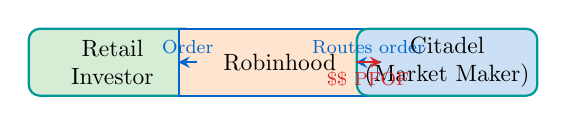
\begin{tikzpicture}[node distance=2.5cm, scale=0.85, transform shape]
\node (user) [blockchain, fill=dfgreen!20, align=center] {Retail\\Investor};
\node (robin) [process, right of=user, fill=dforange!20] {Robinhood};
\node (citadel) [blockchain, right of=robin, fill=dfblue!20, align=center] {Citadel\\(Market Maker)};

\draw[arrow] (user) -- node[above, font=\footnotesize] {Order} (robin);
\draw[arrow] (robin) -- node[above, font=\footnotesize] {Routes order} (citadel);
\draw[arrow, dfred] (citadel) -- node[below, font=\footnotesize] {\$\$ PFOF} (robin);
\end{tikzpicture}
\end{center}
\end{column}
\begin{column}{0.4\textwidth}
\textbf{How it works:}
\begin{enumerate}
\item You place a trade
\item Robinhood sends to Citadel
\item Citadel pays Robinhood
\item Citadel profits from spread
\end{enumerate}
\end{column}
\end{columns}

\vspace{3mm}
\begin{columns}[T]
\begin{column}{0.5\textwidth}
\textbf{Arguments For:}
\begin{itemize}
\item Enables ``free'' trading
\item Price improvement possible
\item Democratizes investing
\end{itemize}
\end{column}
\begin{column}{0.5\textwidth}
\textbf{Arguments Against:}
\begin{itemize}
\item Hidden cost to users
\item Conflict of interest
\item Banned in UK, Canada, EU
\end{itemize}
\end{column}
\end{columns}
\end{frame}

% ==================== SLIDE 21: CASE STUDY STRIPE ====================
\begin{frame}{Case Study: Stripe's Business Model}
\begin{columns}[T]
\begin{column}{0.5\textwidth}
\textbf{Value Proposition:}\\
Developer-first payment infrastructure; ``7 lines of code''

\vspace{3mm}
\textbf{Revenue Model:}
\begin{itemize}
\item 2.9\% + \$0.30 per transaction
\item Plus products: Radar, Atlas, Connect
\item Volume discounts for enterprise
\end{itemize}

\vspace{3mm}
\textbf{Moat:}
\begin{itemize}
\item Developer lock-in (integration effort)
\item Product breadth (one vendor)
\item Brand in tech community
\end{itemize}
\end{column}
\begin{column}{0.5\textwidth}
\begin{block}{Platform Strategy}
\textbf{Land}: Simple payments API\\
\textbf{Expand}: Billing, fraud, treasury, identity, lending\\
\textbf{Lock-in}: Deep integration, switching cost
\end{block}

\vspace{2mm}
\textbf{Network Effects:}
\begin{itemize}
\item Indirect: More merchants $\rightarrow$ better fraud models
\item Data flywheel: Scale improves ML
\item Developer ecosystem: Third-party tools
\end{itemize}
\end{column}
\end{columns}
\end{frame}

% ==================== SLIDE 22: THE DATA FLYWHEEL ====================
\begin{frame}{The Data Flywheel: Compounding Advantage}
\begin{center}
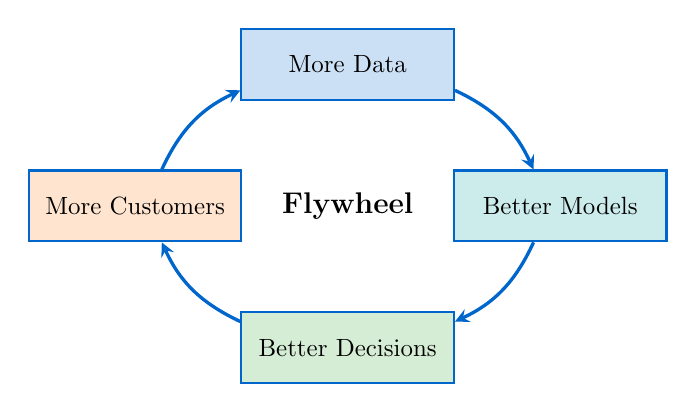
\begin{tikzpicture}[scale=0.9, transform shape]
% Flywheel nodes
\node (data) [process, fill=dfblue!20] at (0,2) {More Data};
\node (model) [process, fill=dfteal!20] at (3,0) {Better Models};
\node (decision) [process, fill=dfgreen!20] at (0,-2) {Better Decisions};
\node (customers) [process, fill=dforange!20] at (-3,0) {More Customers};

% Arrows forming cycle
\draw[arrow, very thick] (data) to[bend left=20] (model);
\draw[arrow, very thick] (model) to[bend left=20] (decision);
\draw[arrow, very thick] (decision) to[bend left=20] (customers);
\draw[arrow, very thick] (customers) to[bend left=20] (data);

% Center label
\node[font=\large\bfseries] at (0,0) {Flywheel};
\end{tikzpicture}
\end{center}

\vspace{3mm}
\textbf{Examples in FinTech:}
\begin{itemize}
\item \textbf{Stripe}: More transactions $\rightarrow$ better fraud detection $\rightarrow$ fewer false positives $\rightarrow$ happier merchants $\rightarrow$ more merchants
\item \textbf{Credit Karma}: More users $\rightarrow$ better credit insights $\rightarrow$ better recommendations $\rightarrow$ more users
\end{itemize}
\end{frame}

% ==================== SLIDE 23: REGULATION AS MOAT ====================
\begin{frame}{Regulation as Moat}
\begin{columns}[T]
\begin{column}{0.5\textwidth}
\textbf{Regulatory Barriers Protect:}
\begin{itemize}
\item Banking charters (capital requirements)
\item Insurance licenses (state-by-state)
\item Broker-dealer registration
\item Money transmitter licenses
\end{itemize}

\vspace{2mm}
\textbf{FinTechs Navigate Via:}
\begin{itemize}
\item BaaS partnerships (rent a charter)
\item Special purpose charters (OCC)
\item Industrial loan companies (Utah)
\item Regulatory arbitrage
\end{itemize}
\end{column}
\begin{column}{0.5\textwidth}
\begin{block}{Regulation as Strategy}
Once compliant, regulation becomes \textbf{moat}:
\begin{itemize}
\item Competitors must also comply
\item Time to license = runway
\item Relationships with regulators valuable
\end{itemize}
\end{block}

\begin{alertblock}{Risk}
Regulatory capture can flip:\\
What protects you can also restrict you
\end{alertblock}
\end{column}
\end{columns}
\end{frame}

% ==================== SLIDE 24: INCUMBENT RESPONSE ====================
\begin{frame}{Incumbent Response: Build, Buy, or Partner}
\begin{center}
\begin{tabular}{p{2.5cm}p{4cm}p{4cm}}
\toprule
\textbf{Strategy} & \textbf{Pros} & \textbf{Cons} \\
\midrule
\textbf{Build} (Internal) & Control, integration & Slow, cultural mismatch \\
\textbf{Buy} (Acquire) & Speed, talent, customers & Expensive, integration risk \\
\textbf{Partner} (API/BaaS) & Fast, low commitment & Dependency, margin sharing \\
\textbf{Copy} (Fast follow) & Proven concept & Behind, no differentiation \\
\textbf{Invest} (Minority stake) & Option value, intel & Limited control \\
\bottomrule
\end{tabular}
\end{center}

\vspace{3mm}
\textbf{Examples:}
\begin{itemize}
\item \textbf{Buy}: JPMorgan acquires InstaMed, WePay, Nutmeg
\item \textbf{Partner}: Goldman + Apple (Apple Card)
\item \textbf{Build}: Chase launches digital-first accounts
\end{itemize}
\end{frame}

% ==================== SLIDE 25: CASE STUDY PAYPAL/VENMO ====================
\begin{frame}{Case Study: PayPal/Venmo}
\begin{columns}[T]
\begin{column}{0.5\textwidth}
\textbf{PayPal (B2C/B2B Payments):}
\begin{itemize}
\item \textbf{Value Prop}: Secure online payments, buyer protection
\item \textbf{Revenue}: Transaction fees (2.9\% + \$0.30)
\item \textbf{Network Effects}: Strong indirect---more merchants = more users
\item \textbf{Moat}: Brand trust, merchant integrations
\end{itemize}

\vspace{3mm}
\textbf{Launch Strategy:}\\
Paid \$10 per signup to reach critical mass quickly
\end{column}
\begin{column}{0.5\textwidth}
\textbf{Venmo (P2P Payments):}
\begin{itemize}
\item \textbf{Value Prop}: Free peer payments, social feed
\item \textbf{Revenue}: Instant transfer fees, business payments
\item \textbf{Network Effects}: Strong direct---value increases with friends on platform
\item \textbf{Moat}: Social graph, habit formation
\end{itemize}

\vspace{3mm}
\begin{block}{Single-Player Mode}
Venmo useful alone for expense tracking, enabling adoption before network effects kick in
\end{block}
\end{column}
\end{columns}
\end{frame}

% ==================== SLIDE 26: CASE STUDY KLARNA ====================
\begin{frame}{Case Study: Klarna (Buy Now, Pay Later)}
\begin{columns}[T]
\begin{column}{0.5\textwidth}
\textbf{Value Proposition:}
\begin{itemize}
\item Consumers: Interest-free installments
\item Merchants: Higher conversion, larger baskets
\end{itemize}

\vspace{3mm}
\textbf{Revenue Model:}
\begin{itemize}
\item Merchant fees: 3-6\% of transaction
\item Late fees from consumers
\item Interest on longer-term financing
\end{itemize}

\vspace{3mm}
\textbf{Network Effects:}
\begin{itemize}
\item Indirect: More merchants $\rightarrow$ more shoppers $\rightarrow$ more merchants
\item Data: Payment history improves risk models
\end{itemize}
\end{column}
\begin{column}{0.5\textwidth}
\begin{alertblock}{Sustainability Questions}
\begin{itemize}
\item Credit losses in economic downturn?
\item Multi-homing: Easy to use Afterpay too
\item Regulatory scrutiny increasing
\item Competition from Apple Pay Later
\end{itemize}
\end{alertblock}

\begin{block}{Assessment}
Strong network effects BUT:
\begin{itemize}
\item Low switching costs for consumers
\item Merchants accept multiple BNPL
\item Credit risk when economy weakens
\end{itemize}
\end{block}
\end{column}
\end{columns}
\end{frame}

% ==================== SLIDE 27: CASE STUDY REVOLUT ====================
\begin{frame}{Case Study: Revolut (Super App Strategy)}
\begin{columns}[T]
\begin{column}{0.5\textwidth}
\textbf{Value Proposition:}\\
All-in-one financial app: banking, crypto, trading, insurance, travel

\vspace{3mm}
\textbf{Revenue Streams:}
\begin{itemize}
\item Subscription tiers (\pounds 0-13/mo)
\item FX markup on free tier
\item Interchange from card spending
\item Crypto trading fees
\item Interest income
\end{itemize}

\vspace{3mm}
\textbf{Growth Strategy:}\\
Land with free FX, expand to full banking
\end{column}
\begin{column}{0.5\textwidth}
\textbf{Network Effects Analysis:}
\begin{itemize}
\item \textbf{Direct}: Limited (P2P payments)
\item \textbf{Data}: Strong (cross-product insights)
\item \textbf{Ecosystem}: Growing (third-party integrations)
\end{itemize}

\vspace{3mm}
\begin{block}{Competitive Moat}
\begin{itemize}
\item Product breadth (one app for everything)
\item Banking license (regulatory moat)
\item Switching costs increase with usage
\item 40M+ users create scale advantages
\end{itemize}
\end{block}
\end{column}
\end{columns}
\end{frame}

% ==================== SLIDE 28: COMPARING FINTECH MOATS ====================
\begin{frame}{Comparing FinTech Competitive Moats}
\begin{center}
\begin{tabular}{p{2.2cm}p{2.2cm}p{2.2cm}p{2.2cm}p{2.2cm}}
\toprule
\textbf{Company} & \textbf{Network Effects} & \textbf{Switching Costs} & \textbf{Data Moat} & \textbf{Regulatory} \\
\midrule
Visa/MC & Very Strong & High & Strong & Strong \\
Stripe & Strong & Very High & Very Strong & Medium \\
Robinhood & Weak & Low & Medium & Medium \\
Klarna & Medium & Low & Strong & Low \\
Revolut & Medium & Medium & Strong & Growing \\
\bottomrule
\end{tabular}
\end{center}

\vspace{5mm}
\begin{block}{Key Insight}
The strongest FinTechs combine \textbf{multiple moats}---network effects alone are not enough if switching is easy.
\end{block}
\end{frame}

% ==================== SLIDE 29: DISCUSSION FRAMEWORK ====================
\begin{frame}{Discussion: Evaluating FinTech Sustainability}
\begin{block}{Framework Questions}
\begin{enumerate}
\item Does this FinTech have \textbf{real network effects}, or just growth?
\item What is the \textbf{unit economics} without subsidies?
\item Are \textbf{switching costs} high enough to retain users?
\item Does the \textbf{data advantage} compound over time?
\item Can incumbents \textbf{copy this} easily?
\item Will \textbf{regulation} help or hurt long-term?
\end{enumerate}
\end{block}

\vspace{3mm}
\textbf{Discussion Exercise}: Apply this framework to analyze:
\begin{itemize}
\item Chime (US neobank)
\item Wise (international money transfer)
\item Plaid (API infrastructure)
\end{itemize}
\end{frame}

% ==================== SLIDE 30: APPLICATION EXERCISE ====================
\begin{frame}{Application: Build Your Own Analysis}
\textbf{Choose a FinTech and complete this assessment:}

\begin{columns}[T]
\begin{column}{0.5\textwidth}
\textbf{1. Business Model:}
\begin{itemize}
\item What problem does it solve?
\item Who pays? Who benefits?
\item What's the revenue model?
\end{itemize}

\vspace{3mm}
\textbf{2. Network Effects:}
\begin{itemize}
\item Direct, indirect, or none?
\item Is there a data flywheel?
\item What's the critical mass?
\end{itemize}
\end{column}
\begin{column}{0.5\textwidth}
\textbf{3. Competitive Position:}
\begin{itemize}
\item What are the switching costs?
\item Can this be easily copied?
\item Is regulation a moat or threat?
\end{itemize}

\vspace{3mm}
\textbf{4. Sustainability Test:}
\begin{itemize}
\item Would customers stay at fair prices?
\item What happens when subsidies end?
\item Is this a winner-take-most market?
\end{itemize}
\end{column}
\end{columns}
\end{frame}

% ==================== SLIDE 31: EXECUTIVE SUMMARY ====================
\begin{frame}{Executive Summary: Key Takeaways}
\begin{enumerate}
\item \textbf{Platforms create value differently}: They orchestrate exchanges rather than produce goods---the most valuable FinTechs are platforms, not pipelines

\item \textbf{Network effects are the goal, but not guaranteed}: Not every FinTech has real network effects---growth without them is just expensive customer acquisition

\item \textbf{Winner-take-most requires specific conditions}: Strong network effects + high switching costs + low multi-homing---without these, competition persists

\item \textbf{Unit economics determine sustainability}: LTV/CAC $>$ 3x, payback $<$ 18 months---venture subsidies mask reality until funding stops

\item \textbf{Multiple moats beat single advantages}: The strongest FinTechs combine network effects, data advantages, switching costs, AND regulatory positioning
\end{enumerate}

\vspace{3mm}
\begin{block}{Core Skill}
Always ask: ``Would this business work at \textit{sustainable} prices without subsidies?''
\end{block}
\end{frame}

% ==================== SLIDE 32: CONCEPT MAP ====================
\begin{frame}{Concept Map: Platform Economics}
\begin{center}
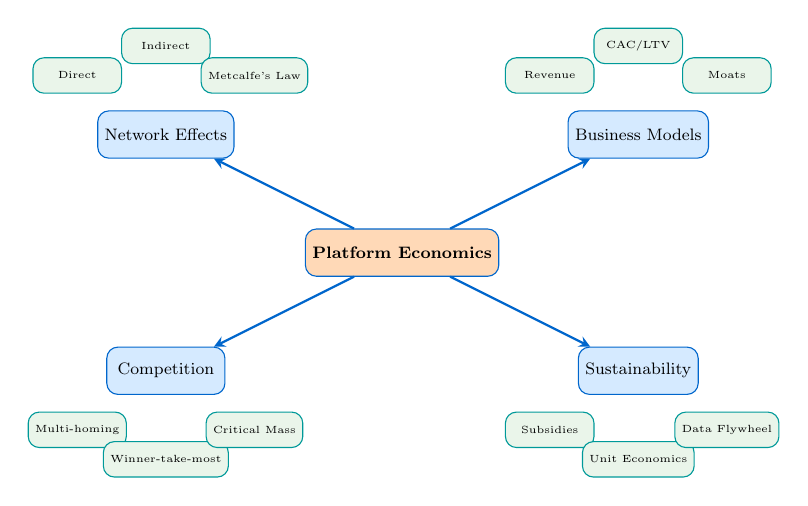
\begin{tikzpicture}[scale=0.75, transform shape,
    concept/.style={rectangle, rounded corners, draw=dfblue, fill=dflightblue4, minimum width=2cm, minimum height=0.8cm, font=\footnotesize},
    subcon/.style={rectangle, rounded corners, draw=dfteal, fill=dfgreen!10, minimum width=1.5cm, minimum height=0.6cm, font=\tiny}]

% Central concept
\node[concept, fill=dforange!30, minimum width=3cm] (platform) at (0,0) {\textbf{Platform Economics}};

% Main branches
\node[concept] (network) at (-4,2) {Network Effects};
\node[concept] (business) at (4,2) {Business Models};
\node[concept] (competition) at (-4,-2) {Competition};
\node[concept] (sustainability) at (4,-2) {Sustainability};

% Connect to center
\draw[arrow] (platform) -- (network);
\draw[arrow] (platform) -- (business);
\draw[arrow] (platform) -- (competition);
\draw[arrow] (platform) -- (sustainability);

% Sub-concepts
\node[subcon] at (-5.5,3) {Direct};
\node[subcon] at (-4,3.5) {Indirect};
\node[subcon] at (-2.5,3) {Metcalfe's Law};

\node[subcon] at (2.5,3) {Revenue};
\node[subcon] at (4,3.5) {CAC/LTV};
\node[subcon] at (5.5,3) {Moats};

\node[subcon] at (-5.5,-3) {Multi-homing};
\node[subcon] at (-4,-3.5) {Winner-take-most};
\node[subcon] at (-2.5,-3) {Critical Mass};

\node[subcon] at (2.5,-3) {Subsidies};
\node[subcon] at (4,-3.5) {Unit Economics};
\node[subcon] at (5.5,-3) {Data Flywheel};

\end{tikzpicture}
\end{center}
\end{frame}

% ==================== SLIDE 33: KEY TERMS 1 ====================
\begin{frame}{Key Terms \& Definitions (1/2)}
\begin{description}
\item[Platform] A business that creates value by facilitating exchanges between two or more interdependent groups

\item[Network Effect] When the value of a product increases as more people use it

\item[Direct Network Effect] Same-side effect: more users = more value for each user (e.g., Venmo)

\item[Indirect Network Effect] Cross-side effect: more users on Side A = more value for Side B (e.g., Visa)

\item[Metcalfe's Law] Network value is proportional to the square of users (n$^2$)

\item[Critical Mass] Minimum users needed for a network to become self-sustaining
\end{description}
\end{frame}

% ==================== SLIDE 34: KEY TERMS 2 ====================
\begin{frame}{Key Terms \& Definitions (2/2)}
\begin{description}
\item[Multi-Homing] Users easily using multiple competing platforms simultaneously

\item[Winner-Take-Most] Market dynamics where one platform captures dominant share

\item[CAC] Customer Acquisition Cost---total spend to acquire one customer

\item[LTV] Lifetime Value---total revenue expected from a customer over time

\item[Data Flywheel] Virtuous cycle: more data $\rightarrow$ better models $\rightarrow$ better service $\rightarrow$ more users $\rightarrow$ more data

\item[Blitzscaling] Strategy of prioritizing growth over efficiency to capture network effects quickly

\item[PFOF] Payment for Order Flow---compensation brokers receive for routing orders to market makers
\end{description}
\end{frame}

% ==================== SLIDE 35: COMMON MISCONCEPTIONS ====================
\begin{frame}{Common Misconceptions: Myth vs. Reality}
\begin{center}
\begin{tabular}{p{5.5cm}p{5.5cm}}
\toprule
\textbf{Myth} & \textbf{Reality} \\
\midrule
``All fast-growing FinTechs have network effects'' & Growth can come from subsidies without any network effects; true network effects make each user more valuable as the network grows \\
\midrule
``Commission-free trading is really free'' & Someone pays---PFOF means market makers pay for order flow; the cost is hidden in execution quality \\
\midrule
``First mover always wins in platforms'' & First mover can lose to better-funded later entrant; what matters is reaching critical mass and building switching costs \\
\midrule
``More features = stronger moat'' & Moats come from network effects, data, and switching costs---not just features that can be copied \\
\bottomrule
\end{tabular}
\end{center}
\end{frame}

% ==================== SLIDE 36: SELF-ASSESSMENT 1 ====================
\begin{frame}{Self-Assessment Questions (1/2)}
\textbf{Question 1:} What is the primary revenue model for Stripe's payment processing service?
\begin{itemize}
\item[A.] Monthly subscription fees only
\item[B.] Payment for order flow (PFOF)
\item[C.] 2.9\% + \$0.30 per transaction
\item[D.] Interest on customer deposits
\end{itemize}

\vspace{5mm}
\textbf{Question 2:} Multi-homing refers to:
\begin{itemize}
\item[A.] Using multiple devices to access a single platform
\item[B.] Users easily using multiple competing platforms simultaneously
\item[C.] Platforms operating in multiple countries
\item[D.] Offering multiple product categories on one platform
\end{itemize}

\vspace{3mm}
\textit{Answers on next slide}
\end{frame}

% ==================== SLIDE 37: SELF-ASSESSMENT 2 ====================
\begin{frame}{Self-Assessment Questions (2/2)}
\textbf{Question 3:} Which condition does NOT typically lead to winner-take-most dynamics?
\begin{itemize}
\item[A.] Strong network effects
\item[B.] Low multi-homing costs
\item[C.] High standardization benefits
\item[D.] Compounding data advantages
\end{itemize}

\vspace{5mm}
\begin{block}{Answers}
\begin{itemize}
\item Question 1: \textbf{C} -- Stripe uses transaction-based pricing at 2.9\% + \$0.30 per transaction
\item Question 2: \textbf{B} -- Multi-homing means users can easily use multiple platforms (e.g., drivers on Uber AND Lyft)
\item Question 3: \textbf{B} -- LOW multi-homing costs prevent tipping because users can switch easily; winner-take-most requires HIGH multi-homing costs
\end{itemize}
\end{block}
\end{frame}

% ==================== SLIDE 38: WHAT'S NEXT ====================
\begin{frame}{What's Next: Day 3 -- Blockchain Fundamentals}
\textbf{Preview of upcoming topics:}

\begin{columns}[T]
\begin{column}{0.5\textwidth}
\textbf{Blockchain Basics:}
\begin{itemize}
\item What is a blockchain?
\item Distributed ledger technology
\item Consensus mechanisms
\item Cryptographic foundations
\end{itemize}

\vspace{3mm}
\textbf{Cryptocurrencies:}
\begin{itemize}
\item Bitcoin and its design
\item Ethereum and smart contracts
\item Token economics
\end{itemize}
\end{column}
\begin{column}{0.5\textwidth}
\textbf{Connection to Platform Economics:}
\begin{itemize}
\item Blockchain platforms have network effects too
\item Ethereum: developer ecosystem effects
\item Token incentives as launch strategy
\item Decentralized platforms vs. centralized
\end{itemize}

\vspace{3mm}
\begin{block}{Key Question}
Can decentralized platforms compete with centralized ones like Visa and Stripe?
\end{block}
\end{column}
\end{columns}
\end{frame}

% ==================== SLIDE 39: RESOURCES ====================
\begin{frame}{Resources for Further Learning}
\textbf{Essential Reading:}
\begin{itemize}
\item Parker, Van Alstyne, Choudary: \textit{Platform Revolution} (2016)
\item Evans \& Schmalensee: \textit{Matchmakers: The New Economics of Multisided Platforms}
\item Cusumano, Gawer, Yoffie: \textit{The Business of Platforms}
\end{itemize}

\vspace{3mm}
\textbf{Academic Papers:}
\begin{itemize}
\item Rochet \& Tirole (2003): ``Platform Competition in Two-Sided Markets''
\item Eisenmann, Parker, Van Alstyne (2006): ``Strategies for Two-Sided Markets''
\end{itemize}

\vspace{3mm}
\textbf{Industry Resources:}
\begin{itemize}
\item a16z FinTech Newsletter (Andreessen Horowitz)
\item Stratechery by Ben Thompson (platform strategy analysis)
\item FinTech company S-1 filings (Robinhood, Coinbase, Affirm)
\end{itemize}
\end{frame}

% ==================== SLIDE 40: QUESTIONS ====================
\begin{frame}
\centering
\vspace{2cm}
{\Huge Questions?}

\vspace{1.5cm}
{\Large Topic 2.4: Platform Economics}

\vspace{1cm}
{\normalsize Network Effects, Winner-Take-Most, and FinTech Business Models}

\vspace{1.5cm}
\textit{``Understanding platform economics is essential for evaluating which innovations are sustainable vs. venture-subsidized.''}
\end{frame}

\end{document}
